\chapter{Tocar m\'usica (MIDI)}
   \label{Tocar-m\'usica}
   \index{Tocar m\'usica} \index{MIDI}

Ya comentamos anteriormente (secci\'on \ref{Menu-Herramientas}) que la versi\'on
para Windows de \texttt{jre} no incorpora las API (\textit{Application Programming
Interface} -- Interfaz de Programaci\'on de Aplicaciones) que contienen los
instrumentos y que deben ser instaladas manualmente (Preguntas frecuentes, 
\ref{Sonido-Instrumentos-Error}). Es importante recordarlo porque, si no lo haces,
con la instalaci\'on por defecto de \textsc{Java} no tendr\'as instrumentos
disponibles. \\

Las primitivas que nos ocupan son:
\begin{center} \begin{longtable}{|m{3.3cm}|c|m{9cm}|} \hline 
   \multicolumn{1}{|c|}{\textbf{Primitivas}} & 
      \multicolumn{1}{c|}{\textbf{Argumentos}} &
         \multicolumn{1}{c|}{\textbf{Uso}} \\ \endhead \hline 
   \texttt{secuencia}, \index{secuencia@\texttt{secuencia}}
      \texttt{sec} \index{sec@\texttt{sec}} & \texttt{a: lista} &
         Carga en memoria la secuencia inclu\'ida en la lista. Siguiendo a
         esta tabla, se indica c\'omo escribir una secuencia de notas
         m\'usicales. \\ \hline 
   \texttt{tocam\'usica} \index{tocam\'usica@\texttt{tocam\'usica}} & \texttt{no} &
         Toca la secuencia de notas en memoria.\\ \hline 
   \texttt{instrumento}, \index{instrumento@\texttt{instrumento}}
      \texttt{instr} \index{instr@\texttt{instr}} & \texttt{no} &
        Da el n\'umero que corresponde al instrumento actualmente seleccionado.
                        \\ \hline 
   \texttt{poninstrumento}, \index{poninstrumento@\texttt{poninstrumento}}
     \texttt{pinstr} \index{pinstr@\texttt{pinstr}} & \texttt{a: n\'umero} &
        Queda seleccionado el instrumento n\'umero \texttt{a}. Puedes ver la
        lista de instrumentos disponibles en el men\'u 
        \textbf{Herramientas $\rightarrow$ Preferencias $\rightarrow$ Sonido}.\\ \hline 
   \texttt{indicesecuencia}, \index{indicesecuencia@\texttt{indicesecuencia}}
      \texttt{indsec} \index{indsec@\texttt{indsec}} & \texttt{no} &
        Da la posici\'on del puntero en la secuencia corriente.\\ \hline 
   \texttt{ponindicesecuencia},
      \index{ponindicesecuencia@\texttt{ponindicesecuencia}}
      \texttt{pindsec} \index{pindsec@\texttt{pindsec}} & 
        \texttt{a: n\'umero}&
        Pone el puntero en la posici\'on \texttt{a} de la secuencia corriente.
                        \\ \hline 
   \texttt{borrasecuencia}, \index{borrasecuencia@\texttt{borrasecuencia}}
     \texttt{bos} \index{bos@\texttt{bos}} & \texttt{no} &
        Elimina de memoria la secuencia corriente.\\ \hline
\end{longtable} \end{center}

Para tocar m\'usica, primero hay que poner en memoria una lista de notas
llamada \textit{secuencia}. Para crear una secuencia, puedes usar
la primitiva \texttt{sec} o \texttt{secuencia}. Para crear una secuencia
v\'alida, hay que seguir las siguientes reglas: 
\begin{itemize}
   \item \texttt{do re mi fa sol la si}: Las notas usuales de la primera
      octava. 
   \item Para hacer un re sostenido, anotamos \texttt{re +} 
   \item Para hacer un re bemol, anotamos \texttt{re -}
   \item Para subir o bajar una octava, usamos \char`\"{}\texttt{:}\char`\"{}
      seguido de \char`\"{}\texttt{+}\char`\"{} o \char`\"{}\texttt{-}\char`\"{}. 
\end{itemize}
\begin{quote}
   \noindent \textbf{Ejemplo}:

   Despu\'es de \texttt{:++} en la secuencia, todas las notas sonar\'an dos
   octavas m\'as altas.
\end{quote}
Por defecto, todas las notas tienen una duraci\'on uno. Si quieres aumentar
o disminuir la duraci\'on, debes escribir un n\'umero correspondiente. \\

\begin{quote}
   \noindent \textbf{Ejemplos}: 
   \begin{verbatim}
      secuencia [sol 0.5 la si] \end{verbatim}
   tocar\'a sol con la duraci\'on 1 y la y si con la duraci\'on 0.5 (el doble
   de r\'apido). \\

   Otro ejemplo:
   \begin{center}
      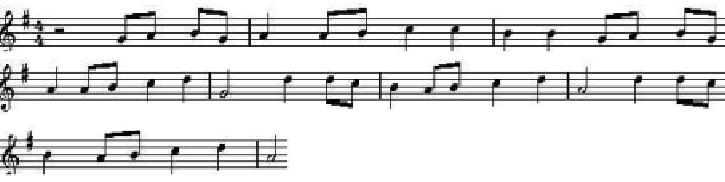
\includegraphics[width=120mm]{Imagenes/09_Musica/musica.png}
   \end{center}
   \begin{verbatim}
 para partitura
 # crea la secuencia de notas
   secuencia [0.5 sol la si sol 1 la 0.5 la si 1 :+ do do :- si si 
      0.5 sol la si sol 1 la 0.5 la si 1 :+ do re 2 :- sol ]
   secuencia [:+ 1 re 0.5 re do 1 :- si 0.5 la si 1 :+ do re 2 :- la ]
   secuencia [:+ 1 re 0.5 re do 1 :- si 0.5 la si 1 :+ do re 2 :- la ]
   secuencia [0.5 sol la si sol 1 la 0.5 la si 1 :+ do do :- si si 
      0.5 sol la si sol 1 la 0.5 la si 1 :+ do re 2 :- sol ]
 fin \end{verbatim}
\end{quote}
Para escuchar la m\'usica, ejecuta las primitivas:

\texttt{partitura tocam\'usica}. \\

\noindent Ahora veamos una aplicaci\'on interesante de la primitiva
\texttt{ponindicesecuencia}: \\

\verb+borrasecuencia # elimina toda secuencia de memoria+ 

\verb+partitura      # pone en memoria las notas+

\verb+pindsec 2      # pone el cursor en el segundo "la"+

\verb+partitura      # pone en memoria las mismas notas, pero movidas 2 lugares.+

\texttt{tocam\'usica}\verb+     # Grandioso!+ \\

\noindent Tambi\'en puedes elegir un instrumento con la primitiva
\texttt{poninstrumento} o en el men\'u \textbf{Herramientas $\rightarrow$
Preferencias $\rightarrow$ Sonido}. Encontrar\'as la lista de instrumentos
disponibles asociados a un n\'umero. (Si usas Windows, echa un vistazo a las
Preguntas Frecuentes si no lo has hecho a\'un) 